% Created 2020-11-09 Mon 12:58
% Intended LaTeX compiler: pdflatex
\documentclass[11pt]{article}
\usepackage[utf8]{inputenc}
\usepackage[T1]{fontenc}
\usepackage{graphicx}
\usepackage{grffile}
\usepackage{longtable}
\usepackage{wrapfig}
\usepackage{rotating}
\usepackage[normalem]{ulem}
\usepackage{amsmath}
\usepackage{textcomp}
\usepackage{amssymb}
\usepackage{capt-of}
\usepackage{hyperref}
\usepackage[english]{babel}
\usepackage[T2A]{fontenc}
\usepackage[utf8]{inputenc}
\usepackage{minted}
\usepackage{wrapfig}
\author{Макаров Сергей, группа 427}
\date{\today}
\title{Контрольная работа №4}
\hypersetup{
 pdfauthor={Макаров Сергей, группа 427},
 pdftitle={Контрольная работа №4},
 pdfkeywords={},
 pdfsubject={},
 pdfcreator={Emacs 27.1 (Org mode 9.4)}, 
 pdflang={English}}
\begin{document}

\maketitle

\section{Задача}
\label{sec:org395a07a}
Удалить мёртвый код в следующей программе:
\begin{center}
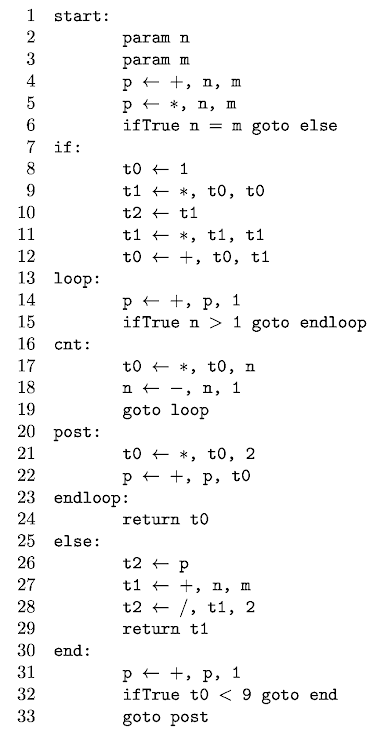
\includegraphics[height=300px]{./code.png}
\end{center}
\pagebreak
\subsection{Решение}
\label{sec:orgdbd128b}
CFG для приведённой программы:
\begin{center}
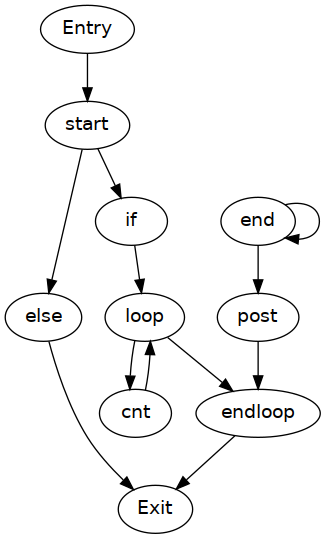
\includegraphics[height=400px]{cfg4.png}
\end{center}

Теперь рассмотрим операции, которые будут помечены на каждой итерации. На первой итерации будут помечены операции \texttt{return t0} в блоке endloop и \texttt{return t1} в блоке \texttt{else}, поскольку эти операции задают возвращаемое значение функции. \(WorkList = \{(return t0), (return t1)\}\)

На второй итерации будут помечены:
\begin{enumerate}
\item \texttt{t1 <- +, n, m} из блока else, т. к. она задаёт определение для t1.
\item \texttt{t0 <- *, t0, 2} из блока post и \texttt{t0 <- +, t0, t1} из блока if, а так же \texttt{t0 <- *, t0, n} из блока cnt, так как они задают определение для t0, достигающее инструкции \texttt{return t0}.
\item \(RDF(endloop) = \{start\}\) и \(RDF(else) = \emptyset\), поэтому помечается также инструкция ветвления в конце блока start.
\item \(WorkList = \{(t1 <- +, n, m), (t0 <- *, t0, 2), (t0 <- *, t0, n), (ifTrue n = m goto else)\}\)
\end{enumerate}

На третьей итерации будут помечены инструкции:
\begin{enumerate}
\item \texttt{param n} и \texttt{param m}, так как они задают определения для m и n, нужные для вычисления \texttt{t1 <- +, n, m}. Кроме того, они же нужны для вычисления ветвления в блоке start, которое было помечено ранее.
\item Инструкция \texttt{t0 <- *, t0, 2} новых пометок не привносит, так как нет достигающих этой инструкции определений переменной t0.
\item Для вычисления инструкции \texttt{t0 <- *, t0, n} из блока cnt нужны определения переменных \texttt{t0} и \texttt{n}, вследствие чего помечается инструкция \texttt{n <- -, n, 1} из того же блока. Единственное неучтённое определение t0 предоставляется этой же инструкцией.
\item Также помечаются инструкции \texttt{t0 <- 1} и \texttt{t1 <- *, t1, t1} из блока if, так как они предоставляют определения переменных t0 и t1, необходимые для инструкции \texttt{t0 <- +, t0, t1}.
\item \(RDF(start) = \emptyset, RDF(if) = \{start\}, RDF(cnt) = \{loop\}\), поэтому так же нужно пометить ветвление в конце start, благо оно уже было помечено, так что в WorkList оно не добавляется. Также помечается ветвление в конце loop.
\item \(WorkList = \{(param n), (param m), (t0 <- 1), (t1 <- *, t1, t1), (n <- -, n, 1), (ifTrue n > 1 goto endLoop)\}\).
\end{enumerate}

Наконец, на последней итерации будет помечена инструкция \texttt{t1 <- *, t0, t0} из блока if, поскольку она предоставляет определение t1, необходимое для инструкции \texttt{t1 <- * t1, t1}. Все остальные инструкции из WorkList новых пометок не провоцируют.

В результате удаления непомеченных инструкций и ветвлений получим код:
\begin{minted}[]{text}
start:
      param n
      param m
      ifTrue n = m goto else
if:
      t0 <- 1
      t1 <- *, t0, t0
      t1 <- *, t1, t1
      t0 <- +, t0, t1
loop:
      ifTrue n > 1 goto endloop
cnt:
      t0 <- *, t0, n
      n <- -, n, 1
      goto loop
post:
      t0 <- *, t0, 2
endloop:
      return t0
else:
      t1 <- +, n, m
      return t1
end:
      goto post
\end{minted}
Заметим, что блоки end и post являются недостижимыми. Ветвление в конце блока end не было помечено, поэтому оно было заменено на переход к ближайшему полезному постдоминатору, т. е. post.
\end{document}
